\documentclass{beamer}

\usepackage{algorithmicx}
\usepackage[lined,vlined,algosection]{algorithm2e}
\usepackage{amsmath, amssymb, amsfonts}
\usepackage{caption}
\usepackage{color}
\usepackage{graphicx}
\usepackage{multirow}
\usepackage{pgfplots}
\usepackage{tikz}
\usetikzlibrary{positioning}
\usepackage{xcolor}

\usetheme{CambridgeUS}

\newcommand{\Field}{\mathbb{F}}
\newcommand{\FField}[1]{\Field_{#1}}
\newcommand{\Ideal}[1]{\langle #1 \rangle}
\newcommand{\LT}[1]{\mathsf{LT}(#1)}
\newcommand{\LM}[1]{\mathsf{LM}(#1)}
\newcommand{\LC}[1]{\mathsf{LC}(#1)}
\newcommand{\Tail}[1]{\mathsf{Tail}(#1)}
\newcommand{\Term}[1]{\mathsf{Term}(#1)}
\newcommand{\Mono}[1]{\mathsf{Mono}(#1)}
\newcommand{\term}{\mathfrak{t}}
\newcommand{\mono}{\mathfrak{m}}
\newcommand{\coef}{\mathfrak{c}}
\newcommand{\mpolyring}[3]{#1[#2_{1}, \ldots, #2_{#3}]}
\newcommand{\LCM}[2]{\mathsf{LCM}(#1, #2)}
\newcommand{\LCMLM}[2]{\LCM{\LM{#1}}{\LM{#2}}}
\newcommand{\Spoly}[2]{\mathsf{Spoly}(#1, #2)}
\newcommand{\Grobner}{Gr\"{o}bner }
\newcommand{\ZZ}{\mathbb{Z}}

\newcommand{\Alg}[2]{\textsc{#1}(#2)}
\newcommand{\FullReduce}[1]{\Alg{FullReduce}{#1}}
\newcommand{\MulFullReduce}[1]{\Alg{MulFullReduce}{#1}}
\newcommand{\GetReductor}[1]{\Alg{GetReductor}{#1}}
\newcommand{\SelectReductor}[1]{\Alg{SelectReductor}{#1}}
\newcommand{\UpdateReduce}[1]{\Alg{UpdateReduce}{#1}}
\newcommand{\Update}[1]{\Alg{Update}{#1}}

\newtheorem{question}{Question}
\newtheorem{link}{}

\title{M4GB: An Efficient \Grobner Bases Algorithm} \author[]{\underline{Rusydi
  H. Makarim}\inst{1, 2} \and Marc Stevens\inst{2}}
\institute[]{\inst{1}Mathematics Institute, University Leiden \and
  \inst{2}Cryptology Group, Centrum Wiskunde en Informatica (CWI)}

\date[]{ISSAC 2017 -- Kaiserslautern, 27th July 2017}

\AtBeginSection[]
{
  \begin{frame}{Table of Contents}
    \tableofcontents[currentsection]
  \end{frame}  
}


\begin{document}

\begin{frame}
  \titlepage
\end{frame}

\begin{frame}{Motivation}
  \begin{block}{Multivariate Quadratic (MQ) Problem}
    Given quadratic polynomials $f_1, \ldots, f_m \in \mpolyring{\Field}{x}{n}$, find a $v = (v_1, \ldots, v_n) \in \Field^n$ such that $f_i (v_1, \ldots, v_n) = 0$ for all $i \in \{ 1, \ldots, m\}$
  \end{block}
  
\end{frame}


\begin{frame}
  \tableofcontents
\end{frame}

\begin{section}{\Grobner Bases Algorithms}
  % Monomial Ordering
  % \begin{frame}{Notations}

  %   \begin{itemize}
  %   \item<2-> $\Field$ - A Field
  %   \item<3-> $\mpolyring{\Field}{x}{n}$ - Polynomial ring over
  %     $\Field$ together with a monomial ordering $<$
  %   \item<4-> For $0 \neq f \in \mpolyring{\Field}{x}{n}$
  %     \begin{itemize}
  %     \item<5-> $\LM{f}, \LC{f}, \LT{f} = \LC{f} \cdot \LM{f}$
  %     \item<5-> $\Tail{f} = f - \LT{f}$
  %     \item<5-> $\Term{f}, \Mono{f}$
  %     \end{itemize}
  %   \item<6-> For $F \subset \mpolyring{\Field}{x}{n}$
  %     \begin{itemize}
  %     \item<7-> $\Ideal{F}$ - Ideal generated by elements of $f$
  %     \item<8-> $\Tail{F} = \cup_{f \in F} \{ \Tail{f} \}$
  %     \item<8-> $\Term{F} = \cup_{f \in F} \Term{f}$
  %     \item<8-> $\Mono{F} = \cup_{f \in F} \Mono{f}$
  %     \end{itemize}
  %   \end{itemize}
  % \end{frame}

  % \begin{frame}{S-polynomial}
  %   \begin{itemize}
  %   \item<2-> $f, g \in \mpolyring{\Field}{x}{n}$ be nonzero
  %     polynomials
  %   \item<3-> $x^{\gamma} = \LCMLM{f}{g}$
  %   \end{itemize}
  %   \begin{block}<4->{Definition}
  %   $$
  %   \Spoly{f}{g} = \dfrac{x^{\gamma}}{\LT{f}} f -
  %   \dfrac{x^{\gamma}}{\LT{g}} g
  %   $$
  % \end{block}
  
  % \begin{columns}[T]
%     \begin{column}{.48\textwidth}
%       \begin{block}<5->{Left}
%         $\textsc{Left}((f, g)) = (x^{\gamma} / \LT{f}, f)$\\
%       \end{block}
%     \end{column}
%     \begin{column}{.48\textwidth}
%       \begin{block}<6->{Right}
%         $\textsc{Right}((f, g)) = (x^{\gamma} / \LT{g}, g)$\\
%       \end{block}
%     \end{column}
%   \end{columns}

%   \onslide<7->{\center{$P \subset \mpolyring{\Field}{x}{n} \times
%       \mpolyring{\Field}{x}{n}$}}

%   \begin{columns}[T]
%     \begin{column}{.48\textwidth}
%       \begin{block}<8->{}
%         $\textsc{Left}(P) = \{ \textsc{Left}(p) : \forall p \in P\}$
%       \end{block}
%     \end{column}
%     \begin{column}{.48\textwidth}
%       \begin{block}<9->{}
%         $\textsc{Right}(P) = \{ \textsc{Right}(p) : \forall p \in P\}$
%       \end{block}
%     \end{column}
%   \end{columns}
% \end{frame}

% \begin{frame}{Polynomial Reduction}
%   \begin{block}<2->{Reductor} Let
%     $0 \neq f \in \mpolyring{\Field}{x}{n}$. A nonzero polynomial
%     $g \in \mpolyring{\Field}{x}{n}$ is a reductor of $f$ if there
%     exists $u \in \Mono{f}$ such that $\LM{g} = u$
%   \end{block}

%   \begin{block}<3->{} $\FullReduce{f, G}$ - Remainder on the division
%     of $f$ by $G \subset \mpolyring{\Field}{x}{n}$
%   \end{block}
% \end{frame}

% \begin{frame}{\Grobner Basis : Definition}
%   \begin{definition}
%     \onslide<2->{$I \neq \{ 0 \}$ be an ideal of $\mpolyring{\Field}{x}{n}$}\\
%     \onslide<3->{$G \subseteq I$, $|G| < \infty$, $\Ideal{G} = I$ is a
%       \Grobner basis of $I$ if,}

%     \onslide<4->{\center{$\forall f \in I$, $\exists g \in G$
%         s.t. $\LT{g} \mid \LT{f}$}}
%   \end{definition}
% \end{frame}

% \begin{frame}{\Grobner Bases Algorithms}
%   \begin{center}
%     \begin{tikzpicture}
%       \node[] (buchberger) {Buchberger's Algorithm}; \node[below =
%       0.05cm of buchberger] () {(1965)}; \node[right = 3cm of
%       buchberger] (F4) {$F_4$}; \node[below = 0.05cm of F4] ()
%       {(1999)}; \node[right = 1cm of F4] (F5) {$F_5$}; \node[below =
%       0.05cm of F5] () {(2002)};

%       \draw[->, blue, thick] (buchberger) -- (F4) ; \draw[->, blue,
%       thick] (F4) -- (F5);

%       \node[above = 1cm of F5, fill = cyan!20] (F5desc)
%       {\tiny{Signature}}; \node[above = 2cm of F4, text width = 125pt,
%       fill = cyan!20] (F4desc) {\tiny{Reduction of multiple
%           S-polynomials by Gaussian elimination on coefficient
%           matrices}};

%       \draw[->, cyan] (F4desc) -- (F4); \draw[->, cyan] (F5desc) --
%       (F5);
%     \end{tikzpicture}
%   \end{center}
% \end{frame}

\begin{frame}{Buchberger's Algorithm (Buchberger, 1965)}
  \textbf{Input} : $F = \{ f_1, \ldots, f_m \} \subset \mpolyring{\Field}{x}{n}$\\
  \textbf{Output} : A \Grobner basis $G$ of $\Ideal{f_1, \ldots, f_m}$

  \begin{enumerate}
  \item<2-> $G \leftarrow F$
  \item<3-> \textbf{repeat}
  \item<4-> \quad $G' \leftarrow G$
  \item<5-> \quad \textbf{for all}
    $(h_1, h_2) \in G' \times G' \mathbf{\ and\ } h_1 \neq h_2$
  \item<6-> \qquad $r \leftarrow \FullReduce{ \Spoly{h_1}{h_2} , G'}$
  \item<7-> \qquad \textbf{if} $r \neq 0$
  \item<8-> \quad \qquad $G \leftarrow G \cup \{ r \}$
  \item<9-> \textbf{until} $G = G'$
  \item<10-> \textbf{return} $G$
  \end{enumerate}
  
  \begin{block}<11->{Improvement} Detect zero reduction in advance --
    Buchberger's 1st and 2nd criterion (e.g. using Gebauer-M\"{o}ller
    installation)
  \end{block}
  
\end{frame}


\begin{frame}{$F_4$ Algorithm (Faug\`{e}re, 1999)}
  \textbf{Input} : $F = \{ f_1, \ldots, f_m \} \subset \mpolyring{\Field}{x}{n}$\\
  \textbf{Output} : A \Grobner basis $G$ of $\Ideal{f_1, \ldots, f_m}$
  \begin{footnotesize}
    \begin{enumerate}
    \item<2-> $G \leftarrow F$, $\tilde{F}_{0}^{+} \leftarrow F$
    \item<3-> $d \leftarrow 0$
    \item<4-> $P \leftarrow \{ ( f_i, f_j ) : f_i, f_j \in F, i > j\}$
    \item<5-> \textbf{while} $P \neq \{ \}$
    \item<6-> \quad $d \leftarrow d + 1$
    \item<7-> \quad $P_d \leftarrow \textsc{Select}(P)$ \qquad \qquad
      \qquad \qquad \qquad \ //$P_d \subseteq P$
    \item<8-> \quad $P \leftarrow P \setminus P_d$
    \item<9-> \quad
      $L_d \leftarrow \textsc{Left}(P_d) \cup \textsc{Right}(P_d)$
    \item<10-> \quad
      $F_d \leftarrow \textsc{SymbPreprocessing}(L_d, G)$ \qquad
      \ //Construction of a coefficient matrix
    \item<11-> \quad
      $\tilde{F}_d \leftarrow \textsc{GaussianElimination}(F_d)$
      \qquad \quad //Main reduction step
    \item<12-> \quad
      $\tilde{F}_{d}^{+} \leftarrow \{ f \in \tilde{F}_d : \LM{f}
      \not\in \LM{F_d} \}$
    \item<13-> \quad \textbf{for} $h \in \tilde{F}_{d}^{+}$
    \item<14-> \qquad $P \leftarrow P \cup \{ (h, g) : g \in G\}$
    \item<15-> \qquad $G \leftarrow G \cup \{ h \}$
    \item<16-> \textbf{return} $G$
    \end{enumerate}
  \end{footnotesize}

  
  
  % \begin{block}<2->{Improvement} Using Gebauer-M\"{o}ller
  %   Installation
  %   and $\textsc{Simplify}$ function
  % \end{block}
\end{frame}

\begin{frame}{Improvement of $F_4$ : \textsc{Simplify} function}
  \begin{itemize}
    
  \item<2-> Replace $uf$ with $u'f'$ s.t. $\LM{uf} = \LM{u'f'}$ where
    $u, u'$ are monomials
  \item<3-> More reductions are already applied on $f'$
  \item<4-> Requires all previously constructed intermediate matrices
    and their corresponding (reduced) row echelon form
  \item<5-> Rewriting reductors
    % \item $|\Mono{\Tail{u'f'}}| \leq |\Mono{\Tail{uf}}|$
    % \item \textsc{Simplify} yields sparser intermediate matrices.
  \end{itemize}
\end{frame}

\begin{frame}{$F_4$ : Advantages and Disadvantages}
  \begin{block}<2->{Advantages}
    \begin{enumerate}
    \item Parallel reduction of S-polynomials with efficient linear
      algebra
    \end{enumerate}
  \end{block}

  \begin{block}<3->{Disadvantages}
    \begin{enumerate}
    \item Normal selection strategy $\Rightarrow$ Many critical pairs
      processed $\Rightarrow$ Large intermediate matrices
    \item The cost of having \textsc{Simplify} function : high memory
      consumption

    \end{enumerate}
  \end{block}
  
\end{frame}



% \begin{frame}{$F_4$ Algorithm : $\textsc{Simplify}$ function}
%   \begin{itemize}
%   \item Input :
%     \begin{enumerate}
%     \item A monomial $u$
%     \item $0 \neq f \in \mpolyring{\Field}{x}{n}$
%     \item All previous intermediate matrices
%       $F_1, F_2, \ldots, F_{d-1}$
%     \end{enumerate}
    
%   \item<2-> Output
%     \begin{enumerate}
%     \item A monomial $u' \leq u$
%     \item A polynomial $f' \in \mpolyring{\Field}{x}{n}$
%     \end{enumerate}
%     such that $\LM{uf} = \LM{u'f'}$.
%   \item<3-> Intuitive idea : more reductions are already applied on
%     $f'$
%   \item<4-> $|\Mono{\Tail{u'f'}}| < |\Mono{\Tail{uf}}| \Rightarrow$ less coefficient in the row of $u'f'$\\
%   \end{itemize}

%   \begin{block}<5->{} \center{$\textsc{Simplify}$ yield sparser
%     intermediate matrices}
%   \end{block}
% \end{frame}
  
\end{section}

% \begin{section}{Background \& Motivation}
  
%   \begin{frame}{Problem}
    
%     \begin{problem}<2->[Multivariate Quadratic(MQ) problem]

%       \begin{itemize}
%       \item<3-> Given :
%         $f_1, \ldots, f_m \in \mpolyring{\Field}{x}{n}$,
%         $\deg(f_i) = 2$
%       \item<4-> Problem : Find a $(v_1, \ldots, v_n) \in \Field^n$
%         such that
%         \begin{align*}
%           f_1(v_1, \ldots, v_n) &= 0\\
%           &\vdots\\
%           f_m(v_1, \ldots, v_n) &= 0
%         \end{align*}
%       \end{itemize}
%     \end{problem}
%   \end{frame}

%   \begin{frame}{Why MQ Problem ?}
%     \begin{itemize}
%     \item<1-> MQ-problem is NP-complete
%     \item<2-> Post-quantum public-key encryption and signature
%       scheme
%     \item<3-> Need to understand its practical difficulty (How ?)
%     \end{itemize}

%     \begin{block}<4->{Open Public Challenge - MQChallenge}
%       \begin{itemize}
%       \item Initiated at 2015
%       \item Random and dense system
%       \item Various parameters
%       \end{itemize}
%     \end{block}
%   \end{frame}

%   \begin{frame}{MQ Challenge Types}
%     \begin{table}
%       \center
%       \begin{tabular}{|c|c|c|c|}
%         \cline{2-4}
%         \multicolumn{1}{c|}{} & \onslide<2->{$\FField{2}$} &
%           %         \onslide<2->{$\FField{2^8}$} &
%           %         \onslide<2->{$\FField{31}$}\\
%           %         \hline
%           %         \multirow{2}{*}{\onslide<3->{$m = 2n$}} &
%           %         \onslide<1->{\Large{I}} &
%           %         \onslide<1->{\Large{II}} &
%           %         \onslide<1->{\Large{III}} \\
%           %         \cline{2-4}
%           %         & \onslide<5->{$n \geq 55$} &
%           %         \onslide<5->{$n \geq 35$} &
%           %         \onslide<5->{$n \geq 34$}\\
%           %         \hline
%           %         \hline
%           %         \multirow{2}{*}{\onslide<4->{$n \approx 1.5m$}}
%           %         & \onslide<1->{\Large{IV}} &
%           %         \onslide<1->{\Large{V}} &
%           %         \onslide<1->{\Large{VI}} \\
%           %         \cline{2-4}
%           %         & \onslide<6->{$m \geq 55$} &
%           %         \onslide<6->{$m \geq 16$} &
%           %         \onslide<6->{$m \geq 16$}\\
%           %         \hline
%     \end{tabular}
%   \end{table}
%   \begin{block}<7->{Parameter Choice}
%     \begin{itemize}
%     \item<8-> Time to solve : at least one month
%     \item<9-> Using Magma 2.19-9
%     \item<10-> CPU Used : \alert{Four 6-cores Intel(R) Xeon(R) CPU
%       E5-4617 @ 2.9GHz} and \alert{1TB of RAM}
%     \end{itemize}
%   \end{block}
%   \onslide<11->{\center{\url{https://www.mqchallenge.org}}}
% \end{frame}
% \end{section}


\begin{section}{M4GB Algorithm}
  
  
  \begin{frame}
    \begin{block}{}
      \begin{itemize}
      \item Let $g$ be a reductor of $f \in \mpolyring{\Field}{x}{n}$
      \item The term of $f$ corresponding to $\LM{g}$ will be
        eliminated
      \item Less monomials in $\Tail{g}$ $\Rightarrow$ less operations
      \end{itemize}
    \end{block}

    \begin{block}<2->{M4GB Main Strategy} \center{The tail of every
        polynomial must be fully reduced}
    \end{block}

  \end{frame}

  % \begin{frame}{Storing Polynomials}
  %   Assume $g_1, \ldots, g_t \in \mpolyring{\Field}{x}{n}$ are
  %   monic\\
  %   \vspace{5mm}
  %   \begin{tikzpicture}
  %     \onslide<2->{ \node[] (g1) {$g_1 = \LM{g_1} + \Tail{g_1}$};
  %     \node[below of = g1] (g2) {$g_2 = \LM{g_2} + \Tail{g_2}$};
  %     \node[below of = g2] (vdots) {$\vdots$}; \node[below of =
  %     vdots] (gt){$g_t = \LM{g_t} + \Tail{g_t}$}; }

  %     \onslide<4->{ \node[right = 2cm of g1] (g1desc)
  %     {\colorbox{orange}{$\LM{g_1}$}
  %     \colorbox{blue!30}{$\Tail{g_1}$}}; \node[right = 2cm of g2]
  %     (g2desc) {\colorbox{orange}{$\LM{g_2}$}
  %     \colorbox{blue!30}{$\Tail{g_2}$}}; \node[below of = g2desc]
  %     (vdots2) {$\vdots$}; \node[right = 2cm of gt] (gtdesc)
  %     {\colorbox{orange}{$\LM{g_t}$}
  %     \colorbox{blue!30}{$\Tail{g_t}$}}; }

  %     \onslide<3->{ \draw[->, thick] (g1) -- (g1desc); \draw[->,
  %     thick] (g2) -- (g2desc); \draw[->, thick] (gt) -- (gtdesc); }

  %     \onslide<5->{ \node[below left of = gtdesc] () {Key};
  %     \node[below right of = gtdesc] () {Value}; }

  %     \onslide<6->{\node[above right = 0.05cm and 1.8cm of vdots2]
  %     ()
  %     {\Large{$= M$}}; }
    
  %   \end{tikzpicture}
  % \end{frame}

  % \begin{frame}
  %   \begin{itemize}
  %   \item $M$ : Associative array that stores all polynomials
  %     \begin{block}{}
  %       For a monomial $u$,
  %       $$
  %       M[u] = \Tail{f}
  %       $$
  %       $\LM{f} = u$ and $f$ is monic
  %     \end{block}
      
  %   \item $L$ : A set of monomials that tells which polynomials that
  %     constitute as minimal basis
  %   \end{itemize}
    
  % \end{frame}

  \begin{frame}{}
    \begin{itemize}
    \item M4GB is an extension of Buchberger's algorithm
    \item<2-> Two main differences :
      \begin{enumerate}
      \item<3-> M4GB Reduction : prioritizes reduction on tail of
        reductors (recursive)
        \begin{itemize}
        \item $\textsc{MulFullReduce}(G, t, f)$
        \end{itemize}
      \item<4-> Reduction on tail of all polynomials using new element
        found in the ideal
        \begin{itemize}
        \item $\textsc{UpdateReduce}(G, P, f)$
        \end{itemize}
      \end{enumerate}
    \end{itemize}
  \end{frame}
  
  % \begin{frame}{Example : Standard Reduction vs M4GB Reduction}
  %   \begin{normalsize}
  %     $\FField{2}[x_1, x_2, x_3, x_4]$ with \emph{degrevlex}
  %     ordering
  %   \end{normalsize}
  %   \vspace{2mm}
  %   \begin{columns}[T]
  %     \begin{column}<2->[T]{.50\textwidth}
  %       \begin{small}
  %         $f = \textcolor<4>{red}{x_1^2 x_2^3} + x_1 x_2^3 x_4 + x_1
  %         x_3^3 + x_1^3 x_4 + x_2 x_3^2 + x_4^2$\\
  %         \onslide<5->{$f = f - g_1 = \textcolor<6,11>{red}{x_1
  %         x_2^3 x_4} + x_1^3 x_4 + x_2 x_3^2$}
  %         \onslide<12->{$f = f - g_4 = x_1^3 x_4 + x_2 x_3^2 + 1$}
  %       \end{small}
  %     \end{column}
  %     \vrule{}
  %     \begin{column}<3->[T]{.50\textwidth}
  %       \begin{small}
  %         $G = \{ g_1, g_2, g_3 \onslide<10->{,
  %         \textcolor<10>{orange}{g_4} } \}$\\
  %         \vspace{2mm}
  %         $g_1 = \textcolor<4>{red}{x_1^2 x_2^3} + x_1 x_3^3 +
  %         x_4^2$\\
  %         \vspace{1mm}
  %         $g_2 = \textcolor<6>{orange}{x_2^3 x_4} + x_2 x_3 + x_3 +
  %         1$\\
  %         \vspace{1mm}
  %         $g_3 = \textcolor<9>{red}{x_1 x_2 x_3} + x_1 x_3$\\
  %         \vspace{1mm}
  %         \onslide<10->{$ \textcolor<10>{orange}{g_4} = x_1g_2 - g_3
  %         = \textcolor<11>{red}{x_1 x_2^3 x_4} + 1$\\}
  %         \vspace{5mm}
  %         \onslide<7->{$x_1 g_2 = x_1 x_2^3 x_4 +
  %         \textcolor<8>{orange}{\textcolor<9>{red}{x_1 x_2 x_3} +
  %         x_1 x_3 + x_1}$\\}
  %       \end{small}
  %     \end{column}
  %   \end{columns}
  %   \center{\onslide<13->{$r = x_1^3 x_4 + x_2 x_3^2 + 1$}}
  % \end{frame}

  \begin{frame}{M4GB Reduction}
    \vspace{-1.5cm}
    \begin{columns}[T]
      \begin{column}[T]{.50\textwidth}
        \begin{scriptsize}
          \center{$\MulFullReduce{G, t, f}$}\\
          \vspace{0.3cm}

          \begin{enumerate}
          \item<2-> $h \leftarrow 0$
          \item<3-> \textbf{for all} $s \in \Term{f}$
          \item<4-> \quad $r \leftarrow t \cdot s$
          \item<5-> \quad \textbf{if}
            $\exists g \in G : \LT{g} \mid r$ \textbf{then}
          \item<6-> \qquad $(G, g) \leftarrow \GetReductor{G, r}$
          \item<7-> \qquad
            $h \leftarrow h - (r / \LT{g}) \cdot \Tail{g}$
          \item<8-> \quad \textbf{else}
          \item<9-> \qquad $h \leftarrow h + r$
          \item<10-> \textbf{return} (G, h)
          \end{enumerate}
          
          % \begin{algorithm}[H]
          %   $h \leftarrow 0$\\
          %   \ForAll{$s \in \Term{f}$} {
          %   $r \leftarrow t \cdot s$\\
          %   \If{$\exists g \in G : \LT{g} \mid r$} {
          %   $(G, g) \leftarrow \GetReductor{G, r}$\\
          %   $h \leftarrow h - (r / \LT{g}) \cdot \Tail{g}$ } \Else
          %   { $h \leftarrow h + r$ } } \Return{$(G, h)$}
          % \end{algorithm}
        \end{scriptsize}
      \end{column}
      \begin{column}[T]{.55\textwidth}
        \begin{scriptsize}
          \onslide<11->{\center{$\GetReductor{G, r}$}} \vspace{0.3cm}

          \begin{enumerate}
          \item<12-> \textbf{if} $\exists g \in G : \LM{g} = \LM{r}$
            \textbf{then}
          \item<13-> \quad \textbf{return} $(G, g)$
          \item<14-> $f \leftarrow \textsc{ReduceSel}(G, r)$
          \item<15->
            $(G, h) \leftarrow \MulFullReduce{G, r / \LT{f},
              \Tail{f}}$
          \item<16-> \textbf{return} $(G \cup \{ r + h \}, r + h)$
          \end{enumerate}
          
          % \begin{algorithm}[H]
          %   \If{$\exists g \in G : \LM{g} = \LM{r}$} {
          %   \Return{$(G, g)$} }
          %   $f \leftarrow \textsc{ReduceSel}(G, r)$\\
          %   $(G, h) \leftarrow \MulFullReduce{G, r/\LT{f},
          %   \Tail{f}}$\\
          %   \Return{$(G \cup \{ r + h\}, r + h)$}
          % \end{algorithm}
        \end{scriptsize}
      \end{column}
    \end{columns}
  \end{frame}

  \begin{frame}
    \center{$\UpdateReduce{G, P, f}$}

    \begin{enumerate}
    \item<2-> $H \leftarrow \{ \LC{f}^{-1} \cdot f \}$
    \item<2-> $S \leftarrow \Mono{\Tail{G \cup H}} \setminus \LM{H}$
    \item<3-> \textbf{while}
      $\exists u \in S : \LM{f}
      \mid u$ \textbf{do}
    \item<4-> \quad Find the largest monomial $u \in S$ s.t. $\LM{f} \mid u$
    \item<5-> \quad
      $(G, h) \leftarrow \MulFullReduce{G, u/\LT{f}, \Tail{f}}$
    \item<6-> \quad $H \leftarrow H \cup \{ u + h\}$
    \item<7-> \quad $S \leftarrow \Mono{\Tail{G \cup H}} \setminus \LM{H}$
    \item<8-> \textbf{while} $H \neq \{ \}$ \textbf{do}
    \item<9-> \quad Select $h \in H$ such that $\LM{h} = \min (\LM{H})$
    \item<10-> \quad $H \leftarrow H \setminus \{ h\}$
    \item<11-> \quad $H \leftarrow \{ g - ch : g \in H, c$ is the
      coefficient of $\LM{h}$ in $\Tail{g} \}$
    \item<12-> \quad $G \leftarrow \{ g - ch : g \in G, c$ is the
      coefficient of $\LM{h}$ in $\Tail{g} \}$
    \item<13-> \quad $G \leftarrow G \cup \{ h \}$
    %\item<13-> $(G, P) \leftarrow \textsc{Update}(G, P, f)$
    %\item<14-> \textbf{return} $(G, P)$
    \end{enumerate}
    
    % \begin{algorithm}[H]
    %   \begin{footnotesize}
    %     $H \leftarrow \{ \LC{f}^{-1} \cdot f \}$\\
        
    %     \vspace{3mm}
    %     \While{$\exists u \in \Mono{\Tail{M \cup H}} \setminus \LM{H}
    %       : \LM{f} \mid u$} {
    %       $u \leftarrow \max \{ u \in \Mono{\Tail{M \cup H}} \setminus \LM{H} : \LM{f} \mid u \}$\\
    %       $(M, h) \leftarrow \MulFullReduce{L, M, u/\LT{f}, \Tail{f}}$\\
    %       $H \leftarrow H \cup \{ u + h\}$\\
    %     } \vspace{3mm} \While{$H \neq \{ \} $} {
    %       Select $h \in H$ such that $\LM{h} = \min \LM{H}$\\
    %       $H \leftarrow H \setminus \{ h \}$\\
    %       $H \leftarrow \{ g - ch : g \in H, c$ is the coefficient of $\LM{h}$ in $\Tail{g} \}$\\
    %       $M \leftarrow \{ g - ch : g \in M, c$ is the coefficient of $\LM{h}$ in $\Tail{g} \}$\\
    %       $M \leftarrow M \cup \{ h \}$\\
    %     }

    %     \vspace{3mm} $(\hat{L}, \hat{P}) \leftarrow \Update{L, P, \LM{f}}$\\
    %     \Return{$(\hat{L}, M, \hat{P})$}
    %   \end{footnotesize}
    % \end{algorithm}
  \end{frame}

  \begin{frame}{Implementation Specific Notes}
    \begin{block}<2->{}
      M4GB is efficient when polynomials in $G$ are maintained based on the uniqueness of their leading monomial i.e., if $f, g \in G$ s.t. $\LM{f} = \LM{g}$ then $f = g$
    \end{block}

    \begin{itemize}
        \item<3-> $M$ : associative array that maintain all polynomials
        \item<4-> $L$ : a set of monomials that mark which polynomials in $M$ that constitute a minimal basis
      \end{itemize}
    
  \end{frame}
  
  
  % \begin{frame}{Advantage of M4GB}
  %   \begin{enumerate}
  %   \item Guarantee tail-reduced polynomials
  %   \item Ideal for processing small batch of critical pairs
  %   \item Uniqueness of reductor (based on leading monomial)
  %   \end{enumerate}
  % \end{frame}
  
\end{section}

\begin{section}{Fukuoka MQ Challenges}
  \begin{frame}{MQ Challenges}
    \begin{itemize}
    \item<2-> A series of open public challenge to solve MQ problems over finite field.
    \item<3-> Random and dense polynomials
    \item<4-> Goal : understand its practical difficulty
    \end{itemize}

    \begin{block}<5->{}
      \center{\url{https://www.mqchallenge.org}}
    \end{block}
  \end{frame}

  \begin{frame}{MQ Challenge Types}
    \begin{table}
      \center
      \begin{tabular}{|c|c|c|c|}
        \cline{2-4}
        \multicolumn{1}{c|}{} & \onslide<2->{$\FField{2}$} &
                                                             \onslide<2->{$\FField{2^8}$} &
                                                                                            \onslide<2->{$\FField{31}$}\\
        \hline
        \multirow{2}{*}{\onslide<3->{$m = 2n$}} &
                                                  \onslide<1->{\Large{I}} &
                                                                            \onslide<1->{\Large{II}} &
                                                                                                       \onslide<1->{\Large{III}} \\
        \cline{2-4}
                              & \onslide<5->{$n \geq 55$} &
                                                            \onslide<5->{$n \geq 35$} &
                                                                                        \onslide<5->{$n \geq 34$}\\
        \hline
        \hline
        \multirow{2}{*}{\onslide<4->{$n \approx 1.5m$}}
                              & \onslide<1->{\Large{IV}} &
                                                           \onslide<1->{\Large{V}} &
                                                                                                          \onslide<1->{\Large{VI}} \\
        \cline{2-4}
                              & \onslide<6->{$m \geq 55$} &
                                                            \onslide<6->{$m \geq 16$} &
                                                                                        \onslide<6->{$m \geq 16$}\\
        \hline
      \end{tabular}
    \end{table}

    \begin{block}<7->{Parameter Choice}
      \begin{itemize}
      \item<8-> Time to solve : at least one month
      \item<9-> Using Magma 2.19-9
      \item<10-> CPU Used : \alert{Four 6-cores Intel(R) Xeon(R) CPU
          E5-4617 @ 2.9GHz} and \alert{1TB of RAM}
      \end{itemize}
    \end{block}
  \end{frame}
\end{section}


\begin{section}{Implementation Results}
  \begin{frame}
    \begin{itemize}
    \item<1-> Implemented using \texttt{C++11}
    \item<2-> Comparison with existing implementations
      \begin{enumerate}
      \item FGb C Interface - Implementation by Jean-Charles
        Faug\`{e}re\footnote<2->{Available at
          \url{http://www-polsys.lip6.fr/~jcf/FGb/C/index.html}}
      \item Magma v2.20-6 - Implementation by Allan Steel
      \item OpenF4 v1.0.1 - Open source implementation by Coladon,
        Vitse and Joux\footnote<2->{Available at
          \url{https://github.com/nauotit/openf4}}.
      \end{enumerate}

    \item<3-> Test cases
      \begin{enumerate}
      \item Dense quadratic polynomials with coefficients in $\FField{31}$
      \item $m = 2n$ and $m = n + 1$.
      \end{enumerate}
      
     
    \end{itemize}
    
  \end{frame}

  \begin{frame}{Benchmark for $m = 2n$ : Ratio}
    \vspace{-3mm}
    \begin{scriptsize}
      \begin{table}
        \begin{tabular}[h]{|c|c|c|c|c|c|}
          \hline
          \multicolumn{2}{|c|}{} &\multicolumn{4}{c|}{CPU time Ratio}\\
          \hline
          $n$ & $m$   & M4GB    & OpenF4  & Magma    & FGb      \\
          \hline
          $20$ & $40$ & \onslide<2->{$1$} & \onslide<3->{$3.61$} & \onslide<4->{$4.07$}  & \onslide<5->{$8.25$}  \\
          $21$ & $42$ & \onslide<2->{$1$} & \onslide<3->{$2.78$} & \onslide<4->{$2.94$}  & \onslide<5->{$5.89$}  \\
          $22$ & $44$ & \onslide<2->{$1$} & \onslide<3->{$2.70$} & \onslide<4->{$3.81$}  & \onslide<5->{$7.35$}  \\
          $23$ & $46$ & \onslide<2->{$1$} & \onslide<3->{$2.15$} & \onslide<4->{$3.00$}  & \onslide<5->{$6.46$}  \\
          $24$ & $48$ & \onslide<2->{$1$} & \onslide<3->{$4.03$} & \onslide<4->{$12.19$} & \onslide<5->{$25.31$} \\
          $25$ & $50$ & \onslide<2->{$1$} & \onslide<3->{-}      & \onslide<4->{$13.93$} & \onslide<5->{$27.2$}  \\
          $26$ & $52$ & \onslide<2->{$1$} & \onslide<3->{-}      & \onslide<4->{$11.83$} & \onslide<5->{$23.20$} \\
          $27$ & $54$ & \onslide<2->{$1$} & \onslide<3->{-}      & \onslide<4->{$8.8$}   & \onslide<5->{$16.49$} \\
          \hline\hline
          \multicolumn{2}{|c|}{} & \multicolumn{4}{c|}{Memory Usage Ratio} \\
          \hline
          $n$ & $m$ & \onslide<6->{M4GB} & \onslide<6->{FGb}    & \onslide<6->{Magma}   & \onslide<6->{OpenF4 }  \\
          \hline
          20 & 40 & \onslide<7->{$1$} & \onslide<8->{$1.53$} & \onslide<9->{$4.96$}  & \onslide<10->{$58.08$}  \\
          21 & 42 & \onslide<7->{$1$} & \onslide<8->{$1.36$} & \onslide<9->{$4.77$}  & \onslide<10->{$54.88$}  \\
          22 & 44 & \onslide<7->{$1$} & \onslide<8->{$2.32$} & \onslide<9->{$3.8$}   & \onslide<10->{$63.57$}  \\
          23 & 46 & \onslide<7->{$1$} & \onslide<8->{$2.32$} & \onslide<9->{$3.35$}  & \onslide<10->{$66.16$}  \\
          24 & 48 & \onslide<7->{$1$} & \onslide<8->{$2.35$} & \onslide<9->{$13.38$} & \onslide<10->{$244.26$} \\
          25 & 50 & \onslide<7->{$1$} & \onslide<8->{$1.88$} & \onslide<9->{$13.4$}  & \onslide<10->{-}        \\
          26 & 52 & \onslide<7->{$1$} & \onslide<8->{$1.38$} & \onslide<9->{$7.57$}  & \onslide<10->{-}        \\
          27 & 54 & \onslide<7->{$1$} & \onslide<8->{$1.2$}  & \onslide<9->{$5.86$}  & \onslide<10->{-}        \\ 
          \hline
        \end{tabular}
        % \begin{tabular}[h]{|c|c|c|c|c|c|}
        %   \hline
        %   \multicolumn{2}{|c|}{} &\multicolumn{4}{c|}{Total CPU time (sec)}\\
        %   \hline
        %   $n$ & $m$   & M4GB    & OpenF4  & Magma    & FGb      \\
        %   \hline
        %   $20$ & $40$ & $57$    & $206$   & $232$    & $470$    \\
        %   $21$ & $42$ & $170$   & $472$   & $500$    & $1002$   \\
        %   $22$ & $44$ & $424$   & $1145$  & $1617$   & $3118$   \\
        %   $23$ & $46$ & $1060$  & $2274$  & $3185$   & $6849$   \\
        %   $24$ & $48$ & $2556$  & $10293$ & $31168$  & $64700$  \\
        %   $25$ & $50$ & $5575$  & -       & $77679$  & $151653$ \\
        %   $26$ & $52$ & $15517$ & -       & $183629$ & $360055$ \\
        %   $27$ & $54$ & $46548$ & -       & $409452$ & $767543$ \\
        %   \hline\hline
        %   \multicolumn{2}{|c|}{} & \multicolumn{4}{c|}{Memory (MB)} \\
        %   \hline
        %   $n$ & $m$ & M4GB & FGb    & Magma   & OpenF4   \\
        %   \hline
        %   20 & 40 & $73$   & $112$  & $362$   & $4240$   \\
        %   21 & 42 & $121$  & $165$  & $577$   & $6640$   \\
        %   22 & 44 & $226$  & $525$  & $859$   & $14368$  \\
        %   23 & 46 & $395$  & $918$  & $1324$  & $26135$  \\
        %   24 & 48 & $663$  & $1561$ & $8873$  & $161945$ \\
        %   25 & 50 & $1471$ & $2765$ & $19719$ & -        \\
        %   26 & 52 & $3328$ & $4607$ & $25197$ & -        \\
        %   27 & 54 & $6799$ & $8180$ & $39845$ & -        \\
        %   \hline
        % \end{tabular}
      \end{table}
    \end{scriptsize}
  \end{frame}

  
  \begin{frame}{Graph for $m = 2n$}
    \vspace{-10mm}
    \begin{center}
      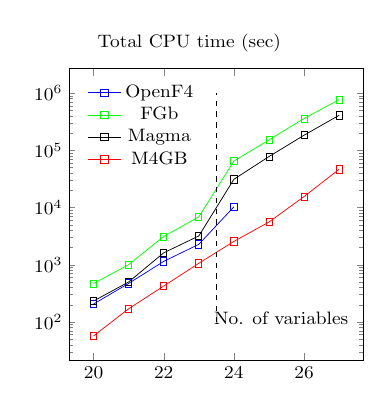
\begin{tikzpicture}[xscale=0.7, yscale=0.65]
        \begin{semilogyaxis}
          [ title={Total CPU time (sec)}, xlabel={No. of variables},
          % ylabel={(sec)},
          x label style={at={(axis description
              cs:.9,0.1)},anchor=south},
          % y label style={at={(axis description
          % cs:0.15,.43)},anchor=north},
          legend pos=north west, legend style={draw=none,fill=none},
          grid style=dashed,
          % scale=0.7 ymin=10,ymax=1000000 xmin=20,xmax=27,
          xscale=0.78 ]
		
          \addplot[color=blue, mark=square]
          coordinates{(20,206)(21,472)(22,1145)(23,2274)(24,10293)};
		
          \addplot[color=green,mark=square]
          coordinates{(20,470)(21,1002)(22,3118)(23,6849)(24,64700)(25,151653)(26,360055)(27,767543)%(28,1578995)
          };
		
          \addplot[color=black,mark=square]
          coordinates{(20,232.16)(21,500.26)(22,1616.73)(23,3184.81)(24,31167.61)(25,77678.58)(26,183628.74)(27,409451.87)%(28,838817.93)
          };
		
          \addplot[color=red,mark=square]
          coordinates{(20,57)(21,170)(22,424)(23,1060)(24,2556)(25,5575)(26,15517)(27,46548)%(28,146204)
          };
        
          \addplot +[mark=none,color=black, style=dashed] coordinates
          {(23.5, 100) (23.5, 1000000)};
          % \node[anchor={north west},rotate=270] at (axis cs:
          % 23.5,1000000) { DoR 5 };
          % \node[anchor={south west},rotate=270] at (axis cs:
          % 23.5,1000000) { DoR 6 };
        
          \legend{OpenF4, FGb, Magma, M4GB}
        \end{semilogyaxis}
        % \draw
      \end{tikzpicture}
      \hspace{10mm}
      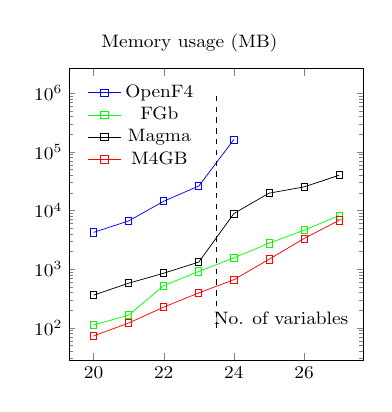
\begin{tikzpicture}[xscale=0.7, yscale=0.65]
        \begin{semilogyaxis}
          [ title={Memory usage (MB)}, xlabel={No. of variables},
          % ylabel={Memory (MB)},
          x label style={at={(axis description
              cs:.9,0.1)},anchor=south},
          % y label style={at={(axis description
          % cs:0.2,.5)},anchor=north},
          legend pos=north west, legend style={draw=none,fill=none},
          grid style=dashed, xscale=0.78 ]
		
          \addplot[color=blue, mark=square]
          coordinates{(20,4240)(21,6640)(22,14368)(23,26135)(24,161945)};
		
          \addplot[color=green,mark=square]
          coordinates{(20,112)(21,165)(22,525)(23,918)(24,1561)(25,2765)(26,4607)(27,8180)%(28,12982)
          };
		
          \addplot[color=black,mark=square]
          coordinates{(20,361.84)(21,577.34)(22,853.84)(23,1324.16)(24,8872.94)(25,19718.78)(26,25197)(27,39844.84)%(28,62790.47)
          };
		
          \addplot[color=red,mark=square]
          coordinates{(20,73)(21,121)(22,226)(23,395)(24,663)(25,1471)(26,3328)(27,6799)%(28,14904)
          };
		
          \addplot +[mark=none,color=black, style=dashed] coordinates
          {(23.5, 100) (23.5, 1000000)};
          % \node[anchor={north west},rotate=270] at (axis cs:
          % 23.5,1500000) { DoR 5 };
          % \node[anchor={south west},rotate=270] at (axis cs:
          % 23.5,1500000) { DoR 6 };
		
          \legend{OpenF4, FGb, Magma, M4GB}
        \end{semilogyaxis}
      \end{tikzpicture}
    \end{center}
  \end{frame}
  
  
  \begin{frame}{Benchmark for $m = n + 1$ : Ratio}
    \vspace{-6mm}
    \begin{footnotesize}
      \begin{table}
        \begin{tabular}[h]{|c|c|c|c|c|c|}
          \hline
          \multicolumn{2}{|c|}{} & \multicolumn{4}{c|}{CPU Time Ratio} \\
          \hline
          $n$  & $m$  & M4GB     & OpenF4   & Magma     & FGb     \\
          \hline
          $10$ & $11$ & \onslide<2->{$1$} & \onslide<3->{$3.05$} & \onslide<4->{$3.36$} & \onslide<5->{$5.1$}  	\\
          $11$ & $12$ & \onslide<2->{$1$} & \onslide<3->{$3.36$} & \onslide<4->{$4.3$}  & \onslide<5->{$8.08$}  \\
          $12$ & $13$ & \onslide<2->{$1$} & \onslide<3->{$2.64$} & \onslide<4->{$4.24$} & \onslide<5->{$9.63$}  \\
          $13$ & $14$ & \onslide<2->{$1$} & \onslide<3->{$2.96$} & \onslide<4->{$4.92$} & \onslide<5->{$11.03$} \\
          $14$ & $15$ & \onslide<2->{$1$} & \onslide<3->{$3.2$}  & \onslide<4->{$7.15$} & \onslide<5->{$14.88$} \\
          $15$ & $16$ & \onslide<2->{$1$} & \onslide<3->{$2.98$} & \onslide<4->{$7.12$} & \onslide<5->{$15$}    \\
          \hline
          \hline
          \multicolumn{2}{|c|}{} & \multicolumn{4}{c|}{Memory Usage Ratio} \\
          \hline
          $n$  & $m$  & \onslide<6->{M4GB}  & \onslide<6->{FGb}    & \onslide<6->{Magma}  &  \onslide<6->{OpenF4}  \\
          \hline
          $10$ & $11$ & \onslide<7->{$1$} & \onslide<8->{$1.94$} & \onslide<9->{$1.88$} &  \onslide<10->{$5.94$}   \\
          $11$ & $12$ & \onslide<7->{$1$} & \onslide<8->{$3.12$} & \onslide<9->{$4$}    &  \onslide<10->{$21.31$}  \\
          $12$ & $13$ & \onslide<7->{$1$} & \onslide<8->{$3.61$} & \onslide<9->{$3.68$} &  \onslide<10->{$47.19$}  \\
          $13$ & $14$ & \onslide<7->{$1$} & \onslide<8->{$4.36$} & \onslide<9->{$3.8$}  &  \onslide<10->{$103$}    \\
          $14$ & $15$ & \onslide<7->{$1$} & \onslide<8->{$4.39$} & \onslide<9->{$4.42$} &  \onslide<10->{$133.84$} \\
          $15$ & $16$ & \onslide<7->{$1$} & \onslide<8->{$4.92$} & \onslide<9->{$3.97$} &  \onslide<10->{$140.26$} \\
          \hline
        \end{tabular}     
      \end{table}
    \end{footnotesize}
  \end{frame}

  \begin{frame}{Graph for $m = n + 1$}
    \vspace{-10mm}
    \begin{center}
      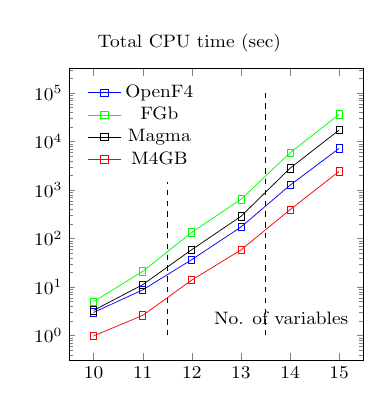
\begin{tikzpicture}[xscale=0.7, yscale=0.65]
        \begin{semilogyaxis}
          [ title={Total CPU time (sec)},%, for the case $m=n+1$.},
          xlabel={No. of variables},
          % ylabel={CPU time (sec)},
          x label style={at={(axis description
              cs:.9,0.1)},anchor=south}, legend pos=north west, legend
          style={draw=none,fill=none}, grid style=dashed, xscale =
          0.78 ] \addplot[color=blue,mark=square] coordinates{(10,
            2.99)(11, 8.73)(12, 36.76)(13, 172.49)(14, 1258)(15,
            7225)};
				
          \addplot[color=green,mark=square]
          coordinates{(10,5)(11,21)(12,134)(13,642)(14,5850)(15,36361)};
		
          \addplot[color=black,mark=square]
          coordinates{(10,3.29)(11,11.172)(12,59.08)(13,286.4)(14,2810.75)(15,17265.5)};
		
          \addplot[color=red,mark=square] coordinates{(10, 0.98)(11,
            2.6)(12, 13.92)(13,58.18)(14, 393.19)(15, 2424)};
		
          \addplot +[mark=none,color=black, style=dashed] coordinates
          {(11.5, 1) (11.5, 1500)};
          % \node[anchor={north west},rotate=270] at (axis cs:
          % 11.5,1500) { DoR 7 };
          % \node[anchor={south west},rotate=270] at (axis cs:
          % 11.5,1500) { DoR 8 };
		
          \addplot +[mark=none,color=black, style=dashed] coordinates
          {(13.5, 1) (13.5, 100000)};
          % \node[anchor={north west},rotate=270] at (axis cs:
          % 13.5,100000) { DoR 8 };
          % \node[anchor={south west},rotate=270] at (axis cs:
          % 13.5,100000) { DoR 9 };
		
          \legend{OpenF4, FGb, Magma, M4GB}
        \end{semilogyaxis}
      \end{tikzpicture}
      \hspace{10mm}
      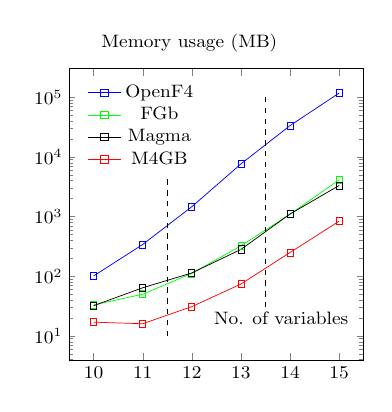
\begin{tikzpicture}[xscale=0.7, yscale=0.65]
        \begin{semilogyaxis}
          [ title={Memory usage (MB)},% for the case $m=n+1$.},
          xlabel={No. of variables}, x label style={at={(axis
              description cs:.9,0.1)},anchor=south},
          % ylabel={Memory (Mbytes)},
          legend pos=north west, legend style={draw=none,fill=none},
          grid style=dashed, xscale = 0.78 ]
          \addplot[color=blue,mark=square]
          coordinates{(10,101)(11,341)(12,1463)(13,7622)(14,33460)(15,117396)};
				
          \addplot[color=green,mark=square]
          coordinates{(10,33)(11,50)(12,112)(13,323)(14,1098)(15,4118)};
		
          \addplot[color=black,mark=square]
          coordinates{(10,32.09)(11,64.12)(12,113.59)(13,281.53)(14,1104)(15,3320)};
		
          \addplot[color=red,mark=square]
          coordinates{(10,17)(11,16)(12,31)(13,74)(14,250)(15,837)};
		
          \addplot +[mark=none,color=black, style=dashed] coordinates
          {(11.5, 10) (11.5, 5000)};
          % \node[anchor={north west},rotate=270] at (axis cs:
          % 11.5,7500) { DoR 7 };
          % \node[anchor={south west},rotate=270] at (axis cs:
          % 11.5,7500) { DoR 8 };
		
          \addplot +[mark=none,color=black, style=dashed] coordinates
          {(13.5, 30) (13.5, 100000)};
          % \node[anchor={north west},rotate=270] at (axis cs:
          % 13.5,180000) { DoR 8 };
          % \node[anchor={south west},rotate=270] at (axis cs:
          % 13.5,180000) { DoR 9 };
		
          \legend{OpenF4, FGb, Magma, M4GB}
        \end{semilogyaxis}
      \end{tikzpicture}
    \end{center}
  \end{frame}
\end{section} %Performance Comparison

\begin{section}{Solving MQ Challenges}
  
  \begin{frame}{Solved MQ Challenges}
    \begin{table}
      \center
      \begin{tabular}{|c|c|c|c|}
        \cline{2-4}
        \multicolumn{1}{c|}{} & $\FField{2}$ & $\FField{2^8}$ & $\FField{31}$\\
        \hline
        \multirow{2}{*}{$m = 2n$} & \Large{I} & \Large{II} & \Large{III} \\
        \cline{2-4}
                              & $n \geq 55$ & $n \geq 35$ & $n \geq 34$\\
        \hline
        \hline
        \multirow{2}{*}{$n \approx 1.5m$} & \Large{IV} & \color<2->{orange}{\Large{V}} &   \color<2->{orange}{\Large{VI}} \\
        \cline{2-4}
                              & $m \geq 55$ & $m \geq 16$ & $m \geq 16$\\
        \hline
      \end{tabular}
    \end{table}
  \end{frame}

  \begin{frame}{Solving Strategy (Bettale, Faug\`{e}re and Perret, 2009)}
    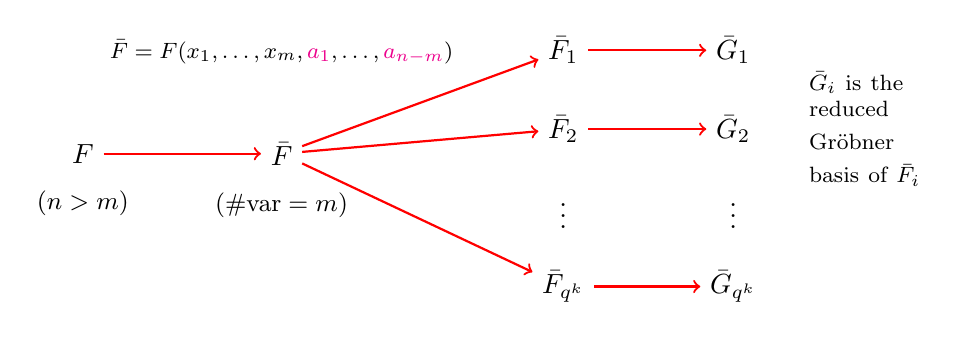
\begin{tikzpicture}
      \node(F){$F$} ; \node [below = 0.1cm of F] (Fparam)
      {\small{$(n > m)$}} ;

      \onslide<2->{\node[right = 2cm of F](Fbar){$\bar{F}$};}
      \onslide<2->{\node[below = 0.1cm of Fbar] (Fbarparam)
        {\small{$(\mathrm{\#var}= m)$}};} \onslide<2->{\node[above =
        0.75cm of Fbar] (Fbarnote)
        {\footnotesize{$\bar{F} = F(x_1, \ldots, x_m,
            \textcolor{magenta}{a_1}, \ldots,
            \textcolor{magenta}{a_{n-m}})$}};}

      
      \onslide<3->{ \node[above right= 0.75cm and 3cm of Fbar] (Fbar1)
        {$\bar{F}_1$}; \node[below of = Fbar1] (Fbar2) {$\bar{F}_2$};
        \node[below of = Fbar2] (vdots) {$\vdots$}; \node[below of =
        vdots] (Fbarqk) {$\bar{F}_{q^k}$};}

      
      \onslide<4->{ \node[right= 1.5cm of Fbar1] (Gbar1)
        {$\bar{G}_1$}; \node[below of = Gbar1] (Gbar2) {$\bar{G}_2$};
        \node[below of = Gbar2] (vdots2) {$\vdots$}; \node[below of =
        vdots2] (Gbarqk) {$\bar{G}_{q^k}$};}


      \onslide<5->{ \node[right = 0.5cm of Gbar2, text width=1.7cm] ()
        {\footnotesize{$\bar{G}_i$ is the reduced\\Gr\"{o}bner basis
            of $\bar{F}_i$}};}

      \onslide<2->{\draw[->, thick, red] (F) -- (Fbar);}
      \onslide<3->{\draw[->, thick, red] (Fbar) -- (Fbar1);}
      \onslide<3->{\draw[->, thick, red] (Fbar) -- (Fbar2);}
      \onslide<3->{\draw[->, thick, red] (Fbar) -- (Fbarqk);}
      \onslide<4->{\draw[->, thick, red] (Fbar1) -- (Gbar1);}
      \onslide<4->{\draw[->, thick, red] (Fbar2) -- (Gbar2);}
      \onslide<4->{\draw[->, thick, red] (Fbarqk) -- (Gbarqk);}

    \end{tikzpicture}

    \begin{block}<6->{} Assume $\bar{F}$ has a unique solution in
      $\FField{q}^{m} \Rightarrow \exists i \in \{ 1, \ldots, q^k\}$
      such that
    $$
    \bar{G}_i = \{ x_1 + \textcolor{orange}{c_1}, \ldots, x_m +
    \textcolor{orange}{c_m} : c_1, \ldots, c_m \in \FField{q}\}
    $$
  \end{block}
  \begin{block}<7->{Solution}
    \center{$(-\textcolor{orange}{c_1}, \ldots,
      -\textcolor{orange}{c_m}, \textcolor{magenta}{a_1}, \ldots,
      \textcolor{magenta}{a_{n-m}}) \in \FField{q}^n$}
  \end{block}
  
  
  
  % \begin{itemize}
  % \item<2-> Hybrid approach
  % \item<3-> Idea :
  %   \begin{enumerate}
  %   \item<4-> Randomly select
  %     $(a_1, \ldots, a_{n-m}) \in \FField{q}^{n-m}$
  %   \item<5-> Construct
    %     $$
    %     \tilde{F} = \{ f(x_1, \ldots, x_m, a_1, \ldots, a_{n-m}) :
    %     \forall f \in F \}
    %     $$
    %   \item<6-> Select small positive integer $k$ (e.g. $1$ or $2$)
    %   \item<7-> Generate $q^k$ subsystems
    %     $$
    %     \{ \tilde{F}(x_1, \ldots, x_{n-k}, v_1, \ldots, v_k) : (v_1,
    %     \ldots, v_k) \in \FField{q}^k\}
    %     $$
    %   \item<8-> Compute \Grobner basis of each subsystem
    %   \end{enumerate}
    % \end{itemize}
\end{frame}

\begin{frame}{Summary of Solved Challenges}
  


  
  \begin{table}
    \begin{tabular}{|c|c|c|c|c|}
      \hline
      Type & $n/m$ & Machine Used & \# Node & Duration \\
      \hline
      \onslide<2->{V} & \onslide<2->{$24/16$} & \onslide<3->{A} & \onslide<3->{$1$} & \onslide<3->{$\approx 9.3$ hours}\\
      \onslide<2->{V} & \onslide<2->{$25/17$} & \onslide<4->{B} & \onslide<4->{$1$} & \onslide<4->{$\approx 46.33$ hours}\\
      \onslide<2->{V} & \onslide<2->{$27/18$} & \onslide<4->{B} & \onslide<4->{$2$} & \onslide<4->{$\approx 10.9$ days}\\
      \hline
      \hline
      \onslide<5->{VI} & \onslide<5->{$24/16$} & \onslide<6->{A} & \onslide<6->{$1$} & \onslide<6->{$\approx 1.2$ hours}\\
      \onslide<5->{VI} & \onslide<5->{$25/17$} & \onslide<7->{B} & \onslide<7->{$1$} & \onslide<7->{$\approx 9.87$ hours}\\
      \onslide<5->{VI} & \onslide<5->{$27/18$} & \onslide<7->{B} & \onslide<7->{$1$} & \onslide<7->{$\approx 31.48$ hours}\\
      \onslide<5->{VI} & \onslide<5->{$28/19$} & \onslide<7->{B} & \onslide<7->{$2$} & \onslide<7->{$\approx 7.61$ days}\\
      \hline
    \end{tabular}
  \end{table}
  \vspace{10mm}
  \begin{footnotesize}
    A) Intel(R) Core(TM) i7-2600K CPU @3.40GHz and 16GB RAM (Desktop)\\
    B) Intel(R) Xeon(R) CPU E5-2650 v3 @ 2.30GHz and 128GB RAM (NUMA)
  \end{footnotesize}
\end{frame}

\begin{frame}{New Record}
  \begin{Large}
    \begin{table}
      \begin{tabular}{|c|c|c|c|c|}
        \hline
        Type & $n/m$ & Machine Used & \# Node & Duration \\
        \hline
        VI & $30/20$ & B & $2$ & $\approx 11.32$ days\\
        \hline
      \end{tabular}
    \end{table}
  \end{Large}
\end{frame}

\end{section} %Solving MQ Challenges

\begin{frame}{Future Work}
  \begin{itemize}
  \item Implementation for sparse system of equations
  \item Vectorization / Parallelization using GPU
  \item Larger finite field
  \item Adapting signature in M4GB
  \end{itemize}
\end{frame}

\begin{frame}
  \center{ \LARGE{ \url{https://github.com/cr-marcstevens/m4gb} }}
\end{frame}

\begin{frame}
  \center{Question ?}
\end{frame}


\end{document}
